
\documentclass[12pt, a4paper, twoside, openright]{book}

\usepackage{vuwthesis} % sets up some local things, mostly the front page

\usepackage{palatino} % sets palatino as the default font

\usepackage{url} % for typesetting urls

\usepackage{graphicx}

\usepackage{listings}

\usepackage{float}

\floatstyle{boxed}
\restylefloat{figure}

%[section] (\usepackage[section]{placeins})

\usepackage[]{algorithm2e}

%\renewcommand{\baselinestretch}{1.00}


\begin{document}

\lstset{language=Java}

\frontmatter
% Book style knows about front matter
% Report style doesn't so you need to set roman numbering etc yourself :-(

%%%%%%%%%%%%%%%%%%%%%%%%%%%%%%%%%%%%%%%%%%%%%%%%%%%%%%%

\title{Maintaining differently refactored views in Java}
\author{Paran Haslett}

\subject{Computer Science}
\abstract{
When developers collaborate on a project there are times when the code diverges. This could be due to refactoring, or the code being reused in another project. It could even be due to throw away code or code used for debugging. This could at times also involve how the structure of the program is presented or the variable and method names that are being used.  In these cases you may need to refactor the code to best suit your changes before you apply them. The ability to have a separate view which although functionally equivalent to other views can present the code in a different form in these situations would be valuable. It enables the programmer to refactor or change the code with minimal impact on others. Changes in the order of of methods and the addition of comments currently impact other developers even if there is no change in how the code works. A tool has been written to detect where source code has been moved within a file or comments has been added removed or edited. This gives us an indication that it would be useful for version control systems to differentiate between changes to a program that also change the behaviour and changes to a program that do not change any behaviour.
}
% Books don't normally have abstracts, and this is a bit of a hack

% Uncomment the appropriate degree
%\phd
\mscthesisonly
%\mscwithhonours
%\mscbothparts
% \otherdegree{DEGREE OR DIPLOMA NAME}



%%%%%%%%%%%%%%%%%%%%%%%%%%%%%%%%%%%%%%%%%%%%%%%%%%%%%%%




\maketitle


\chapter*{Acknowledgments}\label{C:ack} 

I would like to acknowledge the invaluable help of both my supervisors David Pearce and Lindsay Groves and also my wife Hye Eun Park who has been a great support during this thesis.


\tableofcontents


%%%%%%%%%%%%%%%%%%%%%%%%%%%%%%%%%%%%%%%%%%%%%%%%%%%%%%%

% book style knows about mainmatter
% if you are using report style you will have to rest page numbering etc.
\mainmatter

%%%%%%%%%%%%%%%%%%%%%%%%%%%%%%%%%%%%%%%%%%%%%%%%%%%%%%%

% individual chapters included here


\chapter{Introduction}\label{C:intro}

According to Bertino \cite{Bertino2012} \emph{Version control systems} provide a way of allowing multiple developers to collaborate. When multiple developers work on the same source code there is a risk that they have conflicting changes for the same portion of the source code.  One way of managing these conflicting changes is by ensuring only one person can edit a file at a time. This locking mechanism was recommended by Tichy \cite{Tichy1982} for the RCS version control system. Of course, the problem here is that one person can stop others from being able to edit the file. 

An alternative approach is to allow multiple changes to a file and to automatically resolve most of them in a process called a \emph{merge}.  The merge process compares the changes made in one version with the changes made on the other version. If the merge process determines that changes can coexist, it creates a merged file that contains all the changes. The changes that cannot be automatically merged are known as \emph{merge conflicts}.  The merge conflicts need to be manually checked and edited to form a merged file with the correct changes.

\begin{figure}[!t]
 \begin{center}
 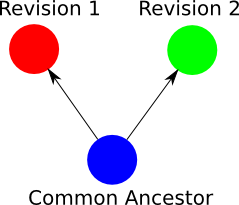
\includegraphics[scale=1]{introRevisions}
 \end{center}
 \caption{A file that has two different revisions}
 \label{fig:introRevisions}
\end{figure}



Internally the merge process needs to determine what changes have happened to both of the revisions being compared. In Figure  ~\ref{fig:introRevisions} there are two revisions that are derived from a common ancestor. It is possible to determine what has been deleted, inserted or changed by comparing each of the revisions against the common ancestor.  This is often done as a linear comparison of the source code for each revision. This works very well provided there has been no change in the order or structure of the file. However, if there has been a change where a block of source code has been moved from one place to another a linear comparison instead determines that two changes have occurred.  This is equivalent to deleting a block of source code from the common ancestor and inserting that source code elsewhere. It is possible that this change is not important to other programmers as the program behaves in the same manner even when source code is in a different order.  An example of this is if a Java programmer changes the order of methods within a program.  The program will behave in the same way as changing the order of methods does not change any functionality, however the source code is now different. The swapping of the order of the method is still counted as being two different changes even though the program behaves in the same manner as it did before the change took place.

Without any further analysis this change is recorded in the merged file even if the reordering was a personal preference for the programmer.  Although there has been no functional change the version control system will treat the relocation of blocks of source code exactly like a change in functionality.  Whenever a programmer attempts to update their code to incorporate any change in functionality, the change to the order of methods is also made to their code.  If a programmer is already familiar with the old structure of code and expects the code to remain relatively consistent the swapping of methods could be disconcerting.

Another issue that non-functional changes raise is an increase in the number of \emph{merge conflicts}. This could occur when two views have had a small amount of refactoring.  Since in both views the behaviour of the program has not changed it is possible that the merge conflict occurs about something trivial. An example of this could be different formatting or ordering methods alphabetically. For an ordinary text merge these changes to the structure of the source code require manual intervention. These issues highlight the need to develop smarter ways to merge.

It is becoming more important to have smarter merges because of the scale of many software projects and the number of developers working on them.
Large online repositories, like GitHub, contain many open source projects.
It is possible for these projects to make source code available to many developers at a time.
This means it is possible for two developers to work on the same project while having little personal contact.
Care needs to be taken when their individual work is combined.
Preferably most of the problems with merging their work should be automatically resolved however,
there still could be instances where either or both developers will have to figure out how the code should interact.
Having better automatic merges reduces the risk that time will be spent manually figuring out how different changes should be combined.

This thesis introduces the concept of maintaining multiple separate views which can be ordered differently but have functionally equivalent source code.
The purpose of these views is to reduce the number of changes introduced during a merge. 
It also explores a way of allowing a version control system to detect when there is a change in the source code but not a functional change in a program.
Examples of this are if items have been reordered, if comments have been inserted or there have been changes to the formatting. 
We developed the Refactor Categories Tool for the purpose of identifying these changes. 
We report on the design and implementation of this tool.
The Refactor Categories Tool is then used in an experiment evaluating a range of real-world benchmarks.


% We have used the Refactor Categories Tool we have created in an experiment 
% that iterates though all the revisions in the version source control for a 
% handful of Java projects.
% The Refactor Categories Tool detects
% 
% need to write about what we found here
 

\section{Overview}
In Chapter 2 we go over the background of version control, the longest common subsequence problem and refactoring as well as look at JDime, an existing tool for merging refactored views.
In Chapter 3 we discuss private views and what they could mean
In Chapter 4 we examine the Refactor Categories Tool, a precursor to developing private view. This will allow us to evaluate if additional merge operations are possible
In Chapter 5 we evaluate the results produced from the Refactor Categories Tool and determine what this could mean for our concept of private views.
In Chapter 6 we will conclude with some future work to make the concept of private view possible. 

% In this thesis we explore the idea of having private views that although 
% functionally equivalent can be refactored differently.
% A version control system allows us to have
% In this thesis we will examine the effects of non functional changes caused 
% by light weight refactoring of code on version control systems.
% To do this we will examine version control systems and how they allow 
% collaboration through merging.
% We will also examine refactoring and how it can change the code but retain 
% the same behaviour.
% We will some tools that could help when merging refactored code when it is 
% checked into an operating system.
% We especially focus on JDime to see if I can help us to build a private view 
% where external code changes are minimised.

\chapter{Background}

As this thesis is about maintaining private views within a version control system what follows is some background concerning version control systems and how they determine if a change has occurred in source code.  
We will also cover refactoring before looking more closely at JDime and other tools that attempt to reduce merge conflicts caused by refactoring or reformatting.  

\section{Version Control Systems}
Version control systems are a way of managing different revisions (or versions). 
Version control systems can be used to keep revisions of files that are in any format. 
Most commonly they are used for maintaining source code written for a plain text programming language (e.g. Java, C, etc.). 
There are a number of reasons why we might want to use a version control system. It can be used to refer to previous revisions, to maintain a revision that has an experimental feature, to associate additional documentation about a feature or to collaborate with multiple developers who are on the same programming project:

\begin{description}

  \item [Revisit revisions using tagging.]
  A version control system can be used by a single person to manage different revisions of their program. 
  A previous revision can always be revisited at a later date and changed. 
  If there is something significant about a particular revision it can be labelled with a \emph{tag}. 
  A tag assigns a name to all the files in the revision you are interested in so that you can more easily revisit the code at a certain point.  
  This is helpful if a software package has a number of released versions.  
  If you need to go back and revisit a particular release it becomes a lot easier if you have tagged the code at that point with the release name or other identification.
   
   

  
  \item [Use branching for experimental features.] 
  It is also possible to maintain multiple revisions of all the files for a software project. 
  This is useful if there is an experimental feature which you want to explore but want to maintain the original as a separate project. 
  As shown in Figure ~\ref{fig:bgBranches} a version control system can keep these multiple interests separate by putting them on different \emph{branches}. 
  It is still possible to easily switch between the different branches depending on which project you want to make changes to.  
  A good use of this feature is if you have a software project that you have written on behalf two different companies but each of them would like their own unique customisations on top of the base product.  
  By making two copies of the base product and having a record of when it was divided the branches can later be recombined to include some or all of the features that have been introduced.  

  \begin{figure}[!t]
   \begin{center}
    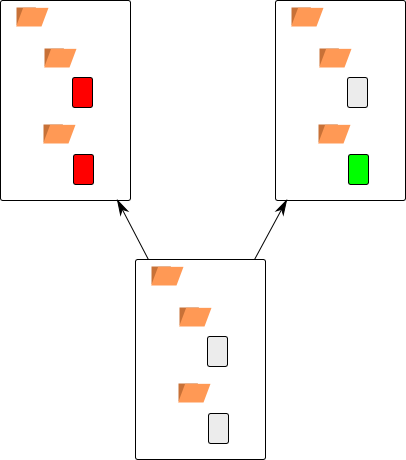
\includegraphics[scale=.8]{branching}
   \end{center}
   \caption{A project that has been split into two branches. Both the red files have been changed for the left branch whilst only the green one has changed in the right branch.}
   \label{fig:bgBranches}
  \end{figure}

  %According to Willaims \cite{Williams2008} branching and merging still is complex and it is hard to get good results from a text-based merge.

  \item [Attach documentation to a feature.]
  Another useful feature of version control is the ability to record meta information beside changes to a set of files.
  The reason this is useful is that you can specify what the change was for.
  It is possible to associate a change that has occurred over multiple files as being for the same reason.
  Most version control systems allow a message to be written when documents are checked in.
  In some version control systems this message is required.
  The reason this is useful is for when queries are made about what a certain change to a document was for.
  Since there is a message beside all the documents about the reason for a particular change it becomes easier to figure out the reason for the individual change we are interested in. 
  % If following the example above we were to examine a document and wonder 
  % why the address changed we could examine the check in with that change and 
  % see the message that the person changing it wrote.

  \begin{figure}[!t]
   \begin{center}
    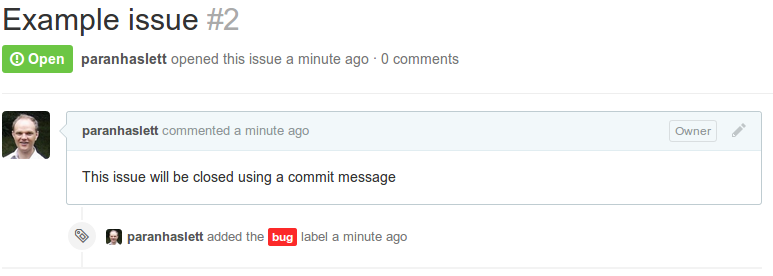
\includegraphics[scale=.5]{bugtrack}
   \end{center}
   \caption{A issue that has been created in GitHub}
   \label{fig:bgBugTrack}
  \end{figure}

  When used on source code in tandem with an \emph{bug tracking system} the message can contain the identification number for the bug being fixed or feature being added.
  This means that anybody who is examining the revision to see the reasoning for the change has access to a lot more information via the bug tracking system.
  An example of this is the \emph{issue tracker} that is built in to GitHub, an online version control system. In GitHub an issue (e.g. a bug report or feature request) can be created as shown in Figure ~\ref{fig:bgBugTrack}. 
  The issue tracker is linked with the messages that you need to write when you check in files.
  If you include a hash sign followed by an issues' identification number in the message you check in then GitHub updates that issue, as shown in Figure ~\ref{fig:bgBugUpdate}.

  \begin{figure}[!t]
   \begin{center}
    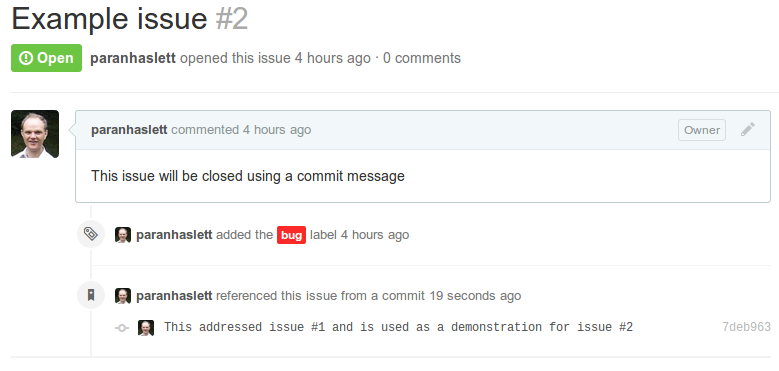
\includegraphics[scale=.5]{bugupdate}
   \end{center}
   \caption{The issue has been updated using a commit message}
   \label{fig:bgBugUpdate}
  \end{figure}

  \item [Collaborate with multiple developers.]
  Version control systems make it possible to have individual revisions that contain each person's changes. 
  The version control system then manages the way these changes are merged into a composite product. 
  Bertino \cite{Bertino2012} describes the ability to merge the work of multiple people as being a powerful collaborative tool. 
  This is because a version control system allows multiple people with different ideas to collaborate on the same document. 
  In some circumstances it allows them to work on the document at the same time. This feature seems similar to the concept of having a private view that we are exploring in this thesis. The difference is that a version control system has no awareness about the format of the documents. This means it is harder for it to evaluate the difference between features of the document that will be helpful to collaboration and features that express the individual tastes of each of the collaborators.

\end{description}



\subsection{Dealing with conflicts}
When people work on the same software project there is a need to interact with each other.
If they require the same source code then there is competition to access that file for each of them to successfully do their work.
There is the risk that they will attempt to change the same block of source code at the same time.
If different changes are made to the same block of source code then they have a \emph{merge conflict} and need to figure out how to combine the changes manually.
There are a few ways of dealing with these conflicts.

\subsubsection{Locking}
One approach is to require that a file is only able to be used by one person at a time and that anyone else has to wait. This method avoids the need to resolve any conflicting changes.  The advantage of locking a file like this is that it is that we can be certain about the contents of the file at any given time. This is how one of the original version control systems, RCS ensured that the document stayed consistent. Tichy \cite{Tichy1982} has explained why he considers locking in a version control system to be a good idea in the design for RCS. The disadvantage is if one person retains the document for extended periods of time, it cannot be changed by anybody else. Furthermore the resulting document may be barely recognisable as the original if extensive work is done on it. However, if the two parties change distinctly different parts of the file, or both independently make exactly the same changes this restriction is unnecessary. 
\subsubsection{Smaller structured units}
Another way to reduce conflicts is to split the programming code into smaller units.  The advantage of this is that if you are using locking you minimise the risk that two people need access to the same unit of source code. Consider two people working on the same project made up of a number of files.  Instead of one person locking a file at a time that person could be allowed to only lock the functions they are changing. As those functions are smaller than the file there is likely to be less changes and they are likely to unlock them sooner.
\subsubsection{Merging documents}
Finally we could allow both parties to change the document and try to figure out what the problems are afterwards.  This resolution of anything that remains a problem is known as resolving a \emph{merge conflict}. This occurs whenever the computer cannot automatically process a merge.  The merge then needs to be sorted out manually. Merge conflicts are more likely to occur if there is a dramatic change such as refactoring.

If not regularly merged it is possible for the source code to diverge greatly and it becomes harder and harder to reconcile.
 According to Bertino it is possible to keep a smaller more easily deployed repository by excluding files that can be generated. \cite{Bertino2012}. Although Bertino refers to unnecessary files this premise may also be applicable for the smaller blocks of code we are interested in. This suggests that maintaining a record about what is relevant and what is irrelevant may have some benefit (e.g. the non-functional changes).
 
\begin{description}
  \item [Manual Merging.]
If you have two files you want to merge but no common starting point for them both you will need to manually merge any differences.
The computer has no record about what the original file looked like so it can not determine which changes were intended.
Features that they have in common will not need to be affected however a decision needs to be made about any differences by the developers responsible for those changes.

% insert diagram
  \item [Automatic Merging.] 
An automatic merge is possible if three revisions are available, the original revision, the revision containing changes we have made and the revision containing changes made by other developers. 
By comparing the differences between our revision and the original one it is possible to determine which changes we have made.  
If we compare the changes made by other developers to the original, the changes that they have made can be determined.  
If we attempt to update our code by merging other people's changes and a change only occurs in our code then that change is retained. 
If we attempt to update our code by merging other people's changes and a change only occurs in the other persons code the the change is inserted into our code.
A merge conflict can however still occur when a change is made in the same area of code in both revisions.
The merge conflicts need to be dealt with manually.


% Diagram showing that how merging could be done automatically
% if there is a change in your code but no change in others code automatic
% if there is a change in others code but not yours
% 
\end{description}
 


%   Version control still can have problems with merge conflicts.

\subsection{Types of version controls systems}
\begin{description}

  \item [Centralised version control.] 
  In a centralised version control system all the changes are made to one location.
  This is called a centralised repository.
  Having a centralised repository means that only one place needs to be checked in order to access the most up-to-date and agreed upon source code.
  The need to be connected to a central system allowed multiple developers the ability to work on the same source code but often had a large overhead.
  Some centralised systems required a specialist to be involved just to look after the server and ensure that merges were done correctly.
  However according to Chacon \cite{Chacon2009} this single point of management has some advantages as it is possible to manage what developers had access to. 
  According to Chacon \cite{Chacon2009} and Bertino \cite{Bertino2012} the main flaw with centralised version control systems is that they have a single point of failure.
  If anything goes wrong with the server you could lose all your work.

  \item [Distributed version control.] 
  According to Chacon \cite{Chacon2009} and Bertino \cite{Bertino2012} this is like having a complete copy of a repository present on every computer that has access to that project

  One advantage of having a complete copy of a project from the repository are that it eliminates the single point of failure that centralised version control systems have.
  It also makes it possible to make changes to the program remotely without being connected to a central server.
  At a later time you are able to merge you changes with other people's work.  
  You are also able to select changes others have made and incorporate them into your personal copy.

  % NOTE: put more in here if time
  \item [Online version control systems.]  
  Whilst is is possible for a measure of collaboration just by using a version control system on its own, it requires that you have some method of obtaining the separate branches on one machine before they can be merged.
  One way of doing this within a company is to set up a server for the version control system.
  This might be suitable for projects that are closed source and have a select group of people who work on the source code.
  For larger projects that have programmers in different parts of the world a publicly accessible version control system that is on the web may be a better solution.
  Loeliger \cite{Loeliger2006} shows how it is possible to access and use a web based version control system to achieve this.
  A good example of a web based version control system is GitHub.
  GitHub provides a way for many developers in different parts of the world to change source code for an open source project.
  It is possible that the developers for a particular project have not even met in real life or even know about each other.

  As an example we could look at the JGit.
  JGit is a pure Java implementation of the Git version control system.
  Figure ~\ref{fig:bgUsage} shows part of the GitHub page for JGit highlighting the amount of activity that there has been on the JGit project.
  With 74 contributors supplying 3245 changes means that the potential to have conflicting changes must be high. Having 20 separate branches may indicate that merges often need to happen. This one example could indicate the need for good merge tools that can reconcile conflicts even if the developers have little contact with each other.

  \begin{figure}[!t]
   \begin{center}
    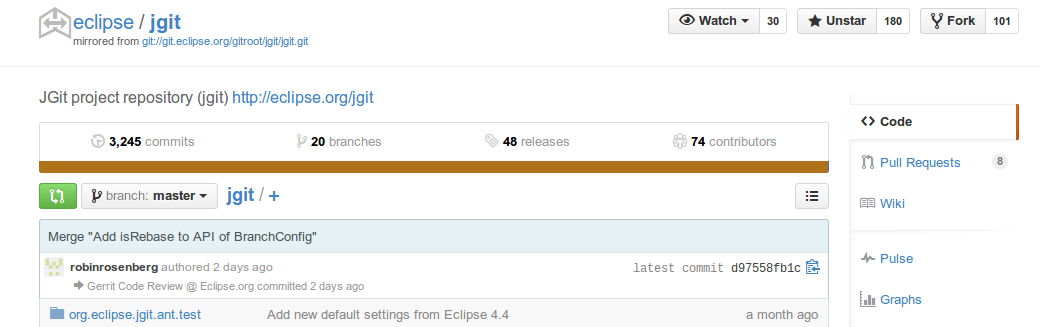
\includegraphics[scale=.47]{githubUsage}
   \end{center}
   \caption{The overview page of the Jgit project in GitHub. This shows that there are 74 contributors to the source code and 3245 individual changes over 20 branches.}
   \label{fig:bgUsage}
  \end{figure}


  
\end{description}

\section{Longest Common Subsequence}
The longest common subsequence problem is relevant to this thesis as it concerns comparing code to determine similarities and differences.
The similarities and differences can then be used to automatically merge code in a version control system.

A simple definition of the longest common subsequence problem is attempting to find the maximum number of common items in two strings when the strings are examined from left to right. A subsequence does not need to be in a single contiguous block however. Algorithms that solve the longest common subsequence can determine the differences between two lists by working out what is the same.   


\subsection{Example}
\label{sec:examplelcs}

An example of finding the longest common subsequence is as follows.
Imagine we have two similar sets of Java source code that we want to compare with each other.  
We would like to know what is the same and what is different.
A longest common subsequence for the source would contain a list of all the lines that are the same and in the same order.


\begin{minipage}[t]{1.0\textwidth}
The first listing is as follows:

%\begin{figure}[!t]
\begin{lstlisting}
public class SampleLCS {
  public static double area(double radius){
    return Math.PI * square(radius);
  }
  
  public static void main(String[] args){
    System.out.println(area(3));
  }
 
  public static double square(double num){
    return num * num;
  }
}
\end{lstlisting}
\end{minipage}
%\end{figure}

\begin{minipage}[t]{1.0\textwidth}
In the second listing the order of a number of methods has changed but the way the code works has not been changed.

%\begin{figure}[!t]
\begin{lstlisting}
public class SampleLCS {
  public static void main(String[] args){
    System.out.println(area(3));
  }
 
  public static double square(double num){
    return num * num;
  }
 
  public static double area(double radius){
    return Math.PI * square(radius);
  }
}
\end{lstlisting}
\end{minipage}
%\end{figure}

\begin{minipage}[t]{1.0\textwidth}
A listing containing only the common lines in the same order between both listings follows.  Since this is one of the longest listings possible it is known as the longest common subsequence.  

%\begin{figure}[!t]
\begin{lstlisting}
public class SampleLCS { 
  public static double area(double radius){
    return Math.PI * square(radius);
  }
  
}
\end{lstlisting}
\end{minipage}
%\end{figure}

\begin{minipage}[t]{1.0\textwidth}
It is possible to have more than one longest common subsequence if there are multiple listings of common lines that have the same number of lines in common and have the maximum number of lines that match.  For instance the following listing is also a longest common subsequence of the above example.

%\begin{figure}[!t]
\begin{lstlisting}
public class SampleLCS {
  public static void main(String[] args){
    System.out.println(area(3));
  }
 
}
\end{lstlisting}
\end{minipage}
%\begin{figure}

As there are possibly multiple longest common subsequences identifying the longest common subsequence that is going to be most useful becomes difficult.

\subsection{Methods of calculating LCS}
According to Arslan \cite{Arslan2010} there are many algorithms that solve longest common subsequence problem. As is it possible for there to be multiple correct solutions to a LCS problem a reason for having a different algorithm may be to find the LCS that make the most intuitive sense. The algorithms used in JGit (an open source implementation of Git in Java) for example are the the Myers, Patience and Histogram algorithms. JGit predominately uses the Histogram algorithm with a fall-back of using the Myers algorithm as a fall-back if it gets to computationally expensive.  There is also the option of using the Patience algorithm however this will produce similar results to the Histogram algorithm which has been derived from it. 

\subsection{Myers}
The Myers algorithm was discovered by Eugene Myers \cite{Myers1986} who claimed that finding the minimal differences between any two documents was the equivalent to finding the shortest or longest path in a graph.

%For example if we have two ...

% explain how this is achieved 

\subsection{Patience}
The patience algorithm instead of figuring out the longest common subsequence directly uses the longest increasing subsequence. 
The example used by Aldous \cite{Aldous1999} to explain how the Patience algorithm finds the longest increasing subsequence is similar to a single player card game.
The aim of the game is to create the minimal number of piles of cards in a row.
A higher card may not be placed on a pile with a lower one in it.
Cards need to be placed on the leftmost valid pile. 
A new pile needs to be created at the end of the row for any cards that cannot be placed on any existing pile.
This game discovers the longest increasing subsequence of the cards when they were shuffled before the game is played.
The cards in the pile to the immediate left of each card when it is played are all possible elements that could come before it in a longest increasing subsequence.
By taking notes of the card on top of of the pile to the immediate left whenever a card is played a longest subsequence can be calculated.     

The Patience algorithm only detects \emph{markers} which are matching lines of code that appear only once in both revisions of the source code.
By using the Patience algorithm on line numbers for the markers instead of on cards the longest common subsequence can be established for those markers. 

As Bram Cohan \cite{bramcohen} has pointed out in his blog there are instances where a traditional LCS algorithm can return results that although correct are not as helpful as they could be.
This is especially true when there are multiple possible longest common subsequences.
The patience algorithm initially ignores lines that appear multiple times and focuses first on solving the longest common subsequence problem for the markers, which only appear once. 
By doing this it has a clearer picture about where to place the lines that occur multiple times.

\subsection{Histogram}
The patience algorithm works well when there are matches that only occur once in both revisions, but has difficulty in determining what to do if line only appear more than once.
It is possible to fall back on a Myers algorithm for the segments where multiple matches occur, however it is possible for Myers to produce unhelpful results. 
The Histogram algorithm attempts to overcome this by also detecting lines that occur in both revisions a small number of times.
The algorithm is solely used in JGit at the moment and is a derivative of the Bram Cohens patience algorithm. 
More details about this algorithm can be found in the Javadoc for HistogramDiff in the JGit source code \cite{Foundation2014}. 


% Before determining a LCS the 

\subsection{How LCS is used in differencing tools}
Differencing tools (often shortened to "diff tools") are programs that compare the contents of two files and show the similarities and differences.
In many diff tools a hash code is assigned to each line of the files to speed up the differencing process.
This means that the differencing tool can work much faster as it does not need to compare each character in the line but can compare hash codes instead.
However the granularity of what is compared is more coarse as it shows complete line differences rather than word or character differences. 
In the source code for many programming languages the white space is not relevant so many diff tools have the option of ignoring the white space and only comparing the code.
This has an impact on the hash codes for each line as the hash code needs to be generated just from the text without including white spaces.

Additionally with some diff tools it is possible to use regular expressions to ignore program features such as comments when doing a diff.  The reason this is important is if it is possible exclude changes that have no affect on behaviour from a diff then it is possible to also exclude them from a merge.  If we exclude them from a merge we could have fewer conflicts.

% insert examples of this with references semantic merge maybe

\subsection{The problem with LCS}
From the perspective of this thesis there is still a problem with longest common subsequence. 
It does not notice changes of order in a document.  
For the example in section \ref{sec:examplelcs} two methods that have swapped positions.
The program still behaves in the same manner when it is run.
It is unnecessary to make any changes to this code in order to get them to behave the same way.
Diff tools that solely use the longest common subsequence do not take different ordered items into account even if they can be considered equivalent.

\begin{figure}[h]
\begin{center}
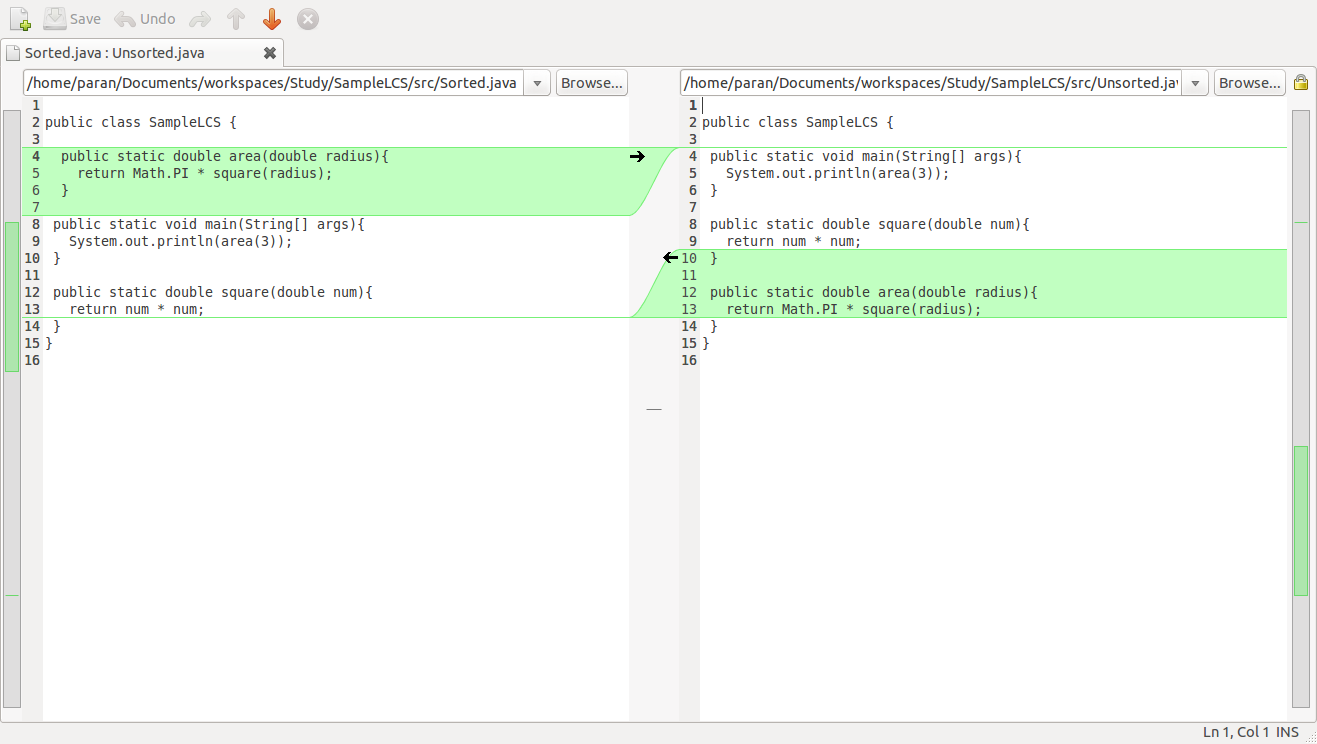
\includegraphics[scale=.28]{lcsDiff}
\end{center}
 \caption{A graphical diff tool showing differences with two equivalent blocks of source code}
\end{figure}


 

\section{Refactoring}
A common concern with coding is the need to periodically refactor the code. 
When we use the word refactored here we refer to the definition of refactoring presented by Murphy-Hill \cite{Murphy-Hill2008} who claims that refactoring simply changes the structure of the code but not the behaviour.
Refactoring simply reorganises the source code so that it is easier to read and add changes. 
According to Fowler et al. the main time for refactoring is when new functionality is added \cite{Fowler1999}. 
Similarly according to Kerievsky some of the motivations for refactoring include adding more code and understanding existing code \cite{Kerievsky2004}.
As adding more functionality is one of the motivations for refactoring let us consider what happens in a multi-developer environment. 
Two developers could have different views on what is considered an appropriate refactoring. 
This is especially true if they need to add different functionality from each other. 
We will now demonstrate this with the following two code examples:

\begin{minipage}[t]{1.0\textwidth}
%\begin{figure}[!t]
\begin{lstlisting}
public TempConv() {
  Scanner keyboard = new Scanner(System.in);
  System.out.println("Enter the temperature in Celsius");
  int celsius = keyboard.nextInt();
  System.out.println("Degrees Fahrenheit is approx " 
    + (celsius * 2 + 30) );
  keyboard.close();
}
\end{lstlisting}
%\end{figure}
\end{minipage}


Refactoring this code depends on what functionality you need to add. 
One developer may recognize that conversion from Celsius may be used several times throughout the code and so extract the calculations as a separate method as follows:

\begin{minipage}[t]{1.0\textwidth}
%\begin{figure}[!t]
\begin{lstlisting}
public TempConv() {
  Scanner keyboard = new Scanner(System.in);
  System.out.println("Enter the temperature in Celsius");
  int celsius = keyboard.nextInt();
  System.out.println("Degrees Fahrenheit is approx " 
    + celsiusToFahrenheit(celsius));
  keyboard.close();
}

public int celsiusToFahrenheit(int celsius){
  return celsius * 2 + 30;
}
\end{lstlisting}
%\end{figure}
\end{minipage}

This change, in spite of producing the same output as the first, provides a number of advantages. Firstly if other programs need to convert from Celsius to Fahrenheit the new method can easily be reused. Secondly since the calculation is a crude estimation it becomes a lot clearer where the code needs to be changed to improve the formula. The ability to add a method that clearly indicates that the calculation is from Celsius to Fahrenheit helps with the readability of the code. There are also disadvantages to doing this refactoring. If we do not care about conversion between Celsius and Fahrenheit the refactoring simply adds to the amount of code we need to examine before understanding what the code does. An alternative way of refactoring is as follows:

\begin{minipage}[t]{1.0\textwidth}
%\begin{figure}[!t]
\begin{lstlisting}
public TempConv(){
  Scanner keyboard = new Scanner(System.in);
  System.out.println("Enter the temperature in Celsius");
  int celsius = keyboard.nextInt();
  int celsiusToFahrenheit = celsius *2 + 30;
  System.out.println("Degrees Fahrenheit is approx " 
    + celsiusToFahrenheit);
  keyboard.close();
}
\end{lstlisting}
%\end{figure}
\end{minipage}

While this again expresses the same functionality as the code above it has not created a new method to do so. This has some of the same advantages. It separates and identifies the formula to convert between Celsius and Fahrenheit. It also uses less code to express this separation than forming a new method. It does not expose the conversion formula outside this method to be used by other calculations however.

As the value of a particular refactoring appears to depend on what is trying to be achieved it is very hard to claim that one refactoring is better than another. Rather, it depends on the wider context of the intention for the refactoring, in this case the level of access required for the approximation to convert Celsius to Fahrenheit.

Although this was a simple example it is easy to imagine a case where a much larger refactoring process is undertaken. In such circumstances a merge becomes difficult. 

\section{JDime}
% Part of the inspiration for this tool come from JDime.

JDime is a tool written by  Apel and Le{\ss}enich \cite{Apel2012} \cite{Apel2011} \cite{LeBenich2012} to study how to get a balance between fast text-based merges and slow but more accurate semantic merges.  JDime is designed to merge two sets of code even if both of them have undergone refactoring. It does this by parsing the class files into AST and evalutating the AST for a \emph{semantic merge} In order to increase performance only if there is a conflict in a text based merge does any of the more expensive semantic merge take place. 

\subsection{How JDime works}
% JDime instead of testing against a source code repository test against files 
% in the system under the base, left and right directories.
% While this may be useful in quickly being able to show what JDime is able to 
% achieve it requires that the inputs need to be previously extracted from a 
% repository into the file system.

Before doing any calculations, JDime runs a regular text merge over the source code.  
If the regular text merge has conflicts then JDime parses the file into an abstract syntax tree (AST).  JDime uses the AST to determine if sections of the source code need to be in a particular order or could be in any order.
What then happens depends on if order is required in the section of code JDime is examining.

% needs more here

\subsection{Investigating JDime}
We performed a small experiment to investigate JDime as a tool for automatically merging code which has been reordered.
% As JDime can examine many refactorings and do comparisons between two 
% private views of source code it is a good contender for allowing us to 
% create two separate views that have different refactorings in them.  However 
% we want the views to remain as consistent as possible. This means we do not 
% want the structure of one view to change the structure of another view if 
% they have the same behaviour when the code is executed.  Any changes to 
% functionality should be able to be communicated between views however 
% changes that are ascetic should not affect the other view.  For this reason 
% we want to test JDimes suitability to be one of the tools used to create 
% separate refactored views.
% 
% JDime has been written mostly in Java.  There are a few exceptions including 
% the linear programming libraries that need to be created.  As we are 
% attempting to combine some of their work with Git it was decided to use JGit 
% rather than the C implementation of Git. As the Java implementation may run 
% a bit slower then in order to get a good timing test running we need to run 
% redo the tests of JDime using JGit instead.
% 
% Also the tests that Le{\ss}enich did on JDime were from files rather than 
% from a repository. It is necessary to set the files back up in the original 
% repository structure to get a adequate baseline.
As JDime performs a type of automatic merge it requires 3 different revisions.
JDime requires a revision that has changes that we want included.  This is commonly called the right revision however I will call this the merger revision as the changes in it are meant to be merged.
JDime also requires a revision that we want to merge into.  This is commonly called the left revision, however I will refer to this as being the mergee. 
Finally JDime requires an original revision that both the merger and the mergee are based on.
This is commonly called the base revision.
% At the moment it cannot access a version control system so each of the 
% revisions need to be set up as directories.
% Each directory needs a full copy of the source code for that revision
% This means that the necessary Java source code to be used by JDime in base, 
% left and right directories.

In order to show how JDime performs extra refactoring based merging we need to attempt to try something that would incorrectly cause a conflict in a text based merge.  The reason that this is necessary is that if there are no conflicts in a text based merge the refactoring aware portion of JDime will not be run.  This saves the overhead of loading the program into an AST in the event that the initial text merge has no conflicts. 
One way to get a lot of text conflicts between two pieces of code that are equivalent when they run is to change the order of the methods.
Although the methods are in different order the programs are still "functionally equivalent".
In order to examine how JDime works and test its suitability a test handler was written.
The test handler creates all of the directories and files for JDime to process.
The methods inside the files are reordered differently for both the left and the right directories.
Figure ~\ref{fig:bgJDimeTest} demonstrates how the test files were arranged.


\begin{figure}[!t]
\begin{center}
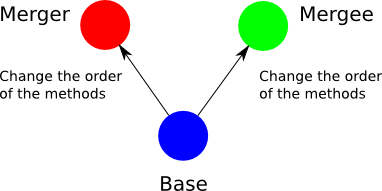
\includegraphics[scale=1]{JdimeTestSetup}
\end{center}
 \label{fig:bgJDimeTest}
 \caption{The set-up for the test of JDime}
\end{figure}

Once the test was set up using the test handler the JDime run to process the directories.
What we expected to happen was that JDime would reorder the methods to match the order in the mergee. As shown in Figure ~\ref{fig:bgJDimeScreenShot} When we compared the methods using a graphical merge tool however we found that the order of the methods in the files did not match.

\begin{figure}[!t]
\begin{center}
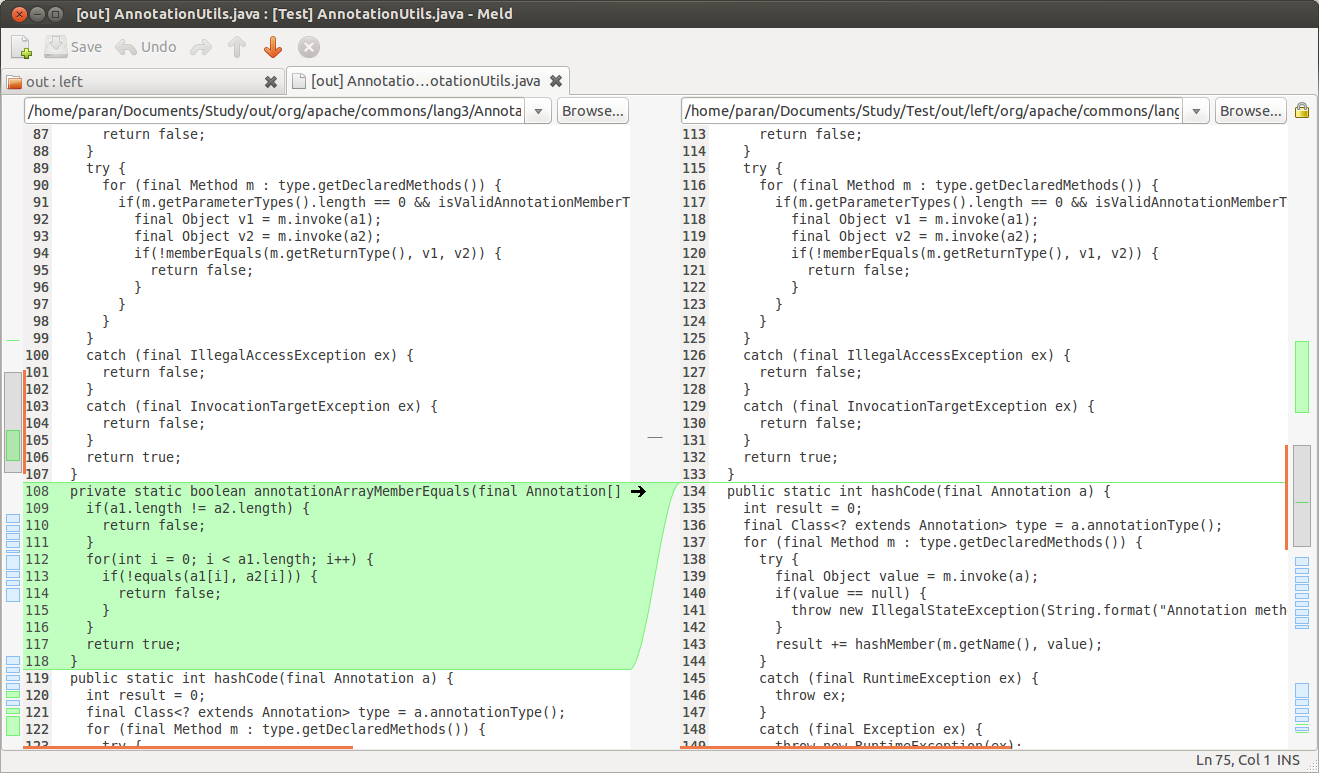
\includegraphics[scale=0.25]{DiffLeft}
\end{center}
 \label{fig:bgJDimeScreenShot}
 \caption{Screen-shot of Meld showing a different method order}
\end{figure}


Further investigation revealed that the order of the methods in the final merged code example did not match the order of any of the equivalent input files.    
In other words JDime normalises its output so that methods are in a particular order.
% If it detects an unordered section it does not preserve the order of the 
% output.

\subsection{Reasons why JDime cannot currently be used to create separate views}
The aim of this thesis is to be able to maintain two views of Java that, although having a different format, function in the same manner.  Although JDime seems like it would be able to help achieve those aims there are a few reasons why it cannot be used without changes.

The first issue is that as explained above that the merged code could be in a totally different order to the original file and both of the revisions.

The second issue is that when JDime parses the code into an AST it strips out any comments or white-space placed in the code.  Although the comments do not have any functional impact on how the program runs they do have an impact on how the source code is understood.  To limit the impact a merge makes on one view comments need to be evaluated as well. In some ways retaining comments or even white-space in the code aids in determining if a section of the code has been copied verbatim from one place to another.


% The only time an AST based merge is performed in JDime is if there are plain 
% text conflicts.  However there could be a hidden conflict that the plain 
% text merge does not detect.  For example if we have two different views and 
% a method has both been relocated in both of them.  Although the method in 
% the original version is in the middle of the code one revision relocates it 
% near to the top of the file and the other to the bottom.  If in addition to 
% this a change is introduced inside the method in both revisions that would 
% normally produce a conflict had the method not been moved.
% 
% A text based merge would not recognise this as a conflict however a AST 
% based one would. According to the text based merge both revisions would 
% agree that the method had been deleted from the middle of the file.  One 
% revision however would insist that a new method with the same name as the 
% deleted one has been created near the top of the file.  The other revision 
% would insist that a new method with the same name had been created but near 
% the bottom. When merged both the method at the top and method at the bottom 
% would be inserted into the merged code.
% 
% A merge using an AST would recognise the methods described as being a 
% conflicting change.  As the names and method signature has not changed for 
% either method it would recognise the conflicting change that has been 
% introduced.
% 
% As JDime does not use an AST comparison to check any items that have been 
% deemed non-conflicting by the text based merge it would miss this conflict.

% According to the text-merge  There could be advantage to determining if 
% items that haven't conflicted in the text based merge but have moved from 
% one position in the code to another.  If a method has both been moved and 
% changed in both branches it could have a conflict.  This conflict would 
% appear to the text-merge as a deletion agreed upon by both branches followed 
% by two insertions at different points.  It would not be picked up by the 
% text-merge as containing a conflict even if one was potentially present.  
% Since the conflict is not detected by a text-merge it is not set aside for 
% testing by examining the AST tree. In this case comparing AST trees could 
% detect that there was a conflict. Although JDime is an improvement over a 
% text-based merge this is a potential conflict that neither detect. There is 
% a performance reason for this design decision. JDime can take a long time to 
% determine if two files contain equivalent source code.

The final concern is that after JDime does the initial comparison of text and finds conflicts it discards those results. It parses the entire file into an AST and begins analysing it again without knowing which parts differ.   

\section{Other refactoring aware versioning tools}
JDime is not the only tool that can be used to address refactor aware version control.  Ekman and Asklund \cite{Ekman2004} introduced a plug-in for eclipse that recorded information about refactoring in to version control so that it was easier to recognise where refactoring took place.  They did this in a very similar manner as Apel and Le{\ss}enich when they developed JDime.  Both make use of an AST to record information about any refactoring that took place.  Freese \cite{Freese2006} also developed a tool that was very similar written in Object-Z. Despite this interest in refactoring aware merges however the idea of maintaining private views has not been discussed.


\chapter{Individual refactored views}

In a project with multiple developers situations may arise where you need to make a change to the structure of the source code. This becomes a problem if you also want to limit the impact other developers.  Maintaining your own independently refactored view of the source code could be valuable in these circumstances. There is a significant amount of interest already in making diff tools and version control systems refactor aware, some examples of this are MolhadoRef \cite{DannyDig} \cite{Dig2008} which attempts to incorporate refactoring in version control systems and commerical systems such as Semantic Merge which is a series of stand alone diff tools for different languages. 

\section{The problem}
\begin{description}
\item [Repeated structure changes for other software developers.]
Imagine a situation where you are working jointly on a project with other people. Since you want to collaborate on different aspects of the same source code you have set up the project in a merge based version control system.  You have checked out your own copy of the code so that you can work on the source code without interfering with any of the changes others are making. You notice that you they are going to have to refactor the code before you add any of your changes.  This would be a fair judgment call as Fowler claims that the main time to do refactoring is before making any changes \cite{Fowler1999}. You complete your changes and check in your code back into the version control system.  While you are doing this other people have been working on the code.  If you manage to check in your code before anyone else you will not need to merge any of your changes.  Anybody who checks in after you however, could have a merge conflict.  Some conflicts that they experience could be because the changes you made directly compete with the changes you have made. Potentially more conflicts would occur between the changes they have made and the refactoring that you have completed. This is because a refactoring often makes a large amount of global changes to the source code.

\begin{figure}
\begin{center}
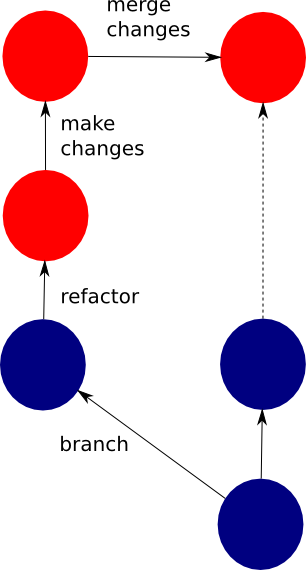
\includegraphics[scale=0.5]{refactorCheckIn}
\end{center}
\caption{Merging changes with refactored code also merges any refactoring}
\end{figure}

As shown in figure the difficulty lies in the fact that not only the functionality that you have added is checked in but also the changes brought about by refactoring.  These refactored changes have not changed how the program functions but have simplified and tidied the code to make the addition of your changes easier. There are some occasions where you may want to avoid changing other peoples code in such a dramatic fashion.

In some conditions refactoring is only required to simplify the code to implement a small change as opposed to cleaning up the entire code base.  This partial refactoring is likely if the code base is large. According to Melina et. al. \cite{Milea2014} refactoring is a challenge when the code base is large. By definition refactoring does not any functionality but changes the source code. This means that the code previous to being partially refactored has the equivalent functionality to the code after the partial refactoring.

By checking in your refactoring code you are forcing others to comply with your vision about how the code should be structured.  This occurs even though you could have no awareness about what changes to the code others have made or intend to make.  Everyone who attempts to check in their code after you will need to merge into a restructured code source that they are unfamiliar with.  The potential for merge based bugs and time wasted doing unnecessary merging increases.

% then created a branch
% If they attempt to check-in their changes there is the possibility a
% conflict with any of your changes.
% 
% You also need to refactor the code to do your work but both of the
% refactorings are different because they clarify or highlight different
% aspects of the source code.
% 
% If there is some refactoring before any changes are made when the code is
% merged with the original project (often called the trunk project) both
% the changes and the refactored code are checked in.
\item [Difficulty if there are multiple check-ins.] 
When there is a large change on a separate branch with many development milestones it is desirable to have the ability to submit your code periodically.  This could be done to ensure that there is not too much divergence between the separate branch and other development projects. The desire to regularly merge the code makes the issue we have discussed even worse. Currently if you have a project where there are periodic check-ins for each development milestone there could be a large impact each time there is a commit. This is because the refactoring for the large refactored project is imposed upon others each time it is merged.

One of the ways this can be dealt with is by creating separate branches for different projects however this has some issues with merging when working on two or more projects simultaneously.  In order to minimize the amount of divergence it is advisable to merge each of the branches with the trunk often.  If there has been global refactoring changes introduced by one project being merged the merge will be worse for any of the remaining branches when they are checked in.  Instead of having an issue merging at the check-in level we now have an issue at the merging of branches.  As these changes will occur less often than checking in the code, the code will possibly have more divergence.  This divergence is likely to cause more rather than less merge issues at the expense of having to merge less often.
\item [Differences in how code is understood.]    
According to  Kerievsky a reason for refactoring code is to better understand it \cite{Kerievsky2004}. As proven by \cite{Bois2005} the very act of going through the source code and reprocessing it in a clearer form can help with the understanding of it. This would suggest that developers tend to leave the code in a difficult to understand state or that different developers understand things differently.
Kerievsky also relates a tale about how the lack of knowledge of patterns making a particular refactoring look a lot more complex \cite{Kerievsky2004}. The different perspectives meant that the programmer he refers to as John has a differing opinion that the refactored code was not an improvement. This shows that it is not just different functionality that influences the need to refactor but sometime the knowledge and experience of the developers themselves. It is often the case that two developers could have different views about what is an appropriate refactoring. This could be because each person brings different skills, notices different issues and has a preferred way of visualizing a problem and solution.
\item [Version control systems not being aware of changes in the order.]
One of the changes which is not catered for by current version control systems is the changes of order.  The first person to check-in their code will have no issue as the version control system assumes that all the changes are simply a new revision.  When the second person attempts to reconcile their view there is the possibility of having unnecessary conflicts.  A lot of these conflicts will be with refactored code which although works the same has a different structure.
\end{description}







\section{Benefits of individual refactored views}
We want to be able to maintain private views or separate branches that can have different but equivalent refactoring. Different structures of code that function the same way a number of features that could be of interest.

\begin{description}

\item [Reduced interference with other software developers.]   
One benefit is that it is possible to keep the structure of code that each software developer works on consistent.  The location of methods and variables are more likely to remain in the place the software developer left them even if a merge occurs.
By maintaining two differently refactored view it allows software developers to work on the same programming project to freely refactor with minimal interference to others.
If two software developers refactor the code that they are able to hold their own individual refactoring with reduced changes when they are merged.
The reduced changes would also mean that there will be less unnecessary merge conflicts when merging code.
  
\item [The number of changes is reduced when merging.] 
The number of changes when merging is reduced if you omit any changes that don't also have any change in behaviour.  This in turn means that there is less chance for there to be a merge conflict.
  
\item [The ability to have comment tied to a specific view.] 
It would be possible to have comments that are not considered when doing a merge. This would be a benefit if there are comment that are specific to a branch and that are not necessary to share.  This would allow a programmer to keep a lot more personal notes.  The risk of having so many comments from others that it is hard to see the code is reduced. By being able to identify that a block of text comment is a new addition

\end{description}

% Can it help with throwaway code or code used for debugging
% 
% When these branches are merged we want to make sure that any source code 
% that is equivalent but refactored is not merged to the view we are merging 
% into. Any source code that changes the behaviour however is considered in 
% the merge.
% 
% We also want to be able to further classify more complex operations in a 
% change set than insert, delete and modify.  When JGit compares files with 
% each other because they are structured it can determine if the file has been 
% moved to a different location in the tree.  At this level JGit can also 
% detect copies and renames.  However once JGit starts comparing source code 
% it loses this structural information.  By giving JGit some idea about the 
% structure in the file it can determine these item at the finer granularity 
% of sections of code rather than at a file basis.


\section{Ways individual refactored views could be achieved}
There are a number of ways we have considered about how to provide differently refactored views that have the same functionality.

\begin{description}
  \item [Comparing differences using a non-ordered comparison algorithm.]   
    Instead of using the Longest Common Sub-sequence (LCS) based approach we could instead use a non-ordered comparison.  The easiest way to consider this concept is that the LCS algorithm compares two lists whereas a non-ordered algorithm is a bit more like comparing sets of items. The items within the set will still be ordered.

    \begin{algorithm}[H]
    \SetAlgoLined
    \While{There are elements on both sides that match}{
    Create a histogram of remaining elements\;
    Select one of the elements that occurs in both sides the least but not zero times\;
    \While{There is an element below the selected one that matches on both sides}{
    Remove element from list of elements to compare, as it matches\;
    }
    \While{There is an element above the selected one that matches on both sides}{
    Remove element from list of elements to compare, as it matches\;
    }
    Remove selected element from list of elements to compare, as it matches\;
    }
    \caption{A non-ordered comparison algorithm}
    \end{algorithm}


    The problems with using this approach to reconcile to different ordered sets is that comparison would not know the difference between what needs to strictly remain in order and what is allowed to be in a different order. If the version control system has an understanding of a particular computer language it is much easier to determine what items can be moved without changing functionality and which ones need to stay in the same order. 
  \item [Normalizing the source code before placing it in the version control system.]
    Before placing the item into source control it could be transformed into an agree upon format. Before allowing a merge on a block of code each the views could transform the block of code using the same method and compare it with the equivalent block of code that in the version control system. If the transformed code is the same then there is no need to merge.
  \item [Storing additional information in the version control system.]
    By storing additional information within the version control system different views could be managed and recreated.
    This concept is very similar to Ekmans plugin for eclipse that maintains a record different refactorings in addition to the source code \cite{Ekman2004}.

    The problem with this is that it would have to store information about every view that was differently refactored.  In a distributed version control system especially an online one the number of distinct views could be large and change often.   
  \item [Using regular expressions]
   It could be possible to use regular experssions to control a lot of the merge process.  We could eliminate a number of comparisons that contain equivalent functionality in this manner.
  \item [Using a tool like JDime solely as a method of comparison.]
    As mentioned earlier there are a number of reasons why JDime cannot currently be used as a method of keeping two different refactored views. If changed however it could still be useful.  One idea we had was to attach it to Git and solely use it to detect equivalent pieces of java source code.
\end{description}

\section{Are comments important?}
Although in this thesis we have focused mostly on changes to the behaviour of a program as opposed to astetic changes to the source code we recognise that sometimes changes to comments may be important.  If a new comment is inserted in a branch or even if a comment is deleted it is likely that the change is specifc to the task the programmer is trying to implement.  However if an existing comment is modified it is more likely that the comment and the task will have some impact on other branches and should be modified.  There could be exceptions where inserted or deleted code should have an impact on other code and where a modification to a comment does not really need to be broadcast to other users during a merge.

Existing comments and even white space can also provide useful information about any changes of order in the code.  If a programmer has cut and pasted a block of code the white space and comments are also moved and provide hints to what has occured.  Even if some of the code has been modified there could be enough clues left behind to suggest that the most likely event is that the code has moved and then adjusted.



\chapter{Refactor Categories Tool}
In order to prove that having private views would provide some useful results we created the Refactor Categories Tool. Version control systems such a JGit compare and merge file by differentiating between insert, delete and modify  opperations. The Refactor Categories Tool enhances this by also including instances where a block of code has moved but the function equivlency remains the same. It also can differentiate between changes to comments, white space and Java code. This means it can differentiate between instances where a change to a source file causes a change in the behaviour of the program and some instances where it has been refactored. When we use the word refactored here we refer to the definition of refactoring presented by Murphy-Hill \cite{Murphy-Hill2008} who claims that refactoring simply changes the structure of the code but not the behaviour. Although it does not detect more complex differences beyond this we intend to show that changes exist in real world software projects that have no impact on the projects' behaviour.



\section{Overview}
The test we use with the Refactor Categories Tool analyses all the historical changes ever made on a software project by extracting successive revisions from a Git repository using JGit.
An ordinary text comparison is used as a starting point.  The algorithm used for the text comparison is the histogram LCS one normally used by JGit with white space ignored. The text comparison returns the minimal number of text changes in an \lstinline{EditList} object.  The \lstinline{EditList} contains a list of changes to the plain text. The information about each change that the \lstinline{EditList} object retains are:

\begin{itemize}
  \item the starting line of the change for both revisions being compared
  \item The ending line of the change for both revisions 
  \item The type of change that is being made
\end{itemize}

The types of changes that are detected between two files are limited to inserts, deletes, and modifications. In order to expand this list we need more information.  We obtain information about the meaning of Java files by parsing both revisions we are comparing into an AST using JastAddJ. We then need to discover which AST node matches which change to the source code. 

Each of the AST nodes contains information about the line of source the AST node starts and ends at.  Unlike the \lstinline{EditList} object which we have previously discussed, an AST node can also hold the column that the AST node starts and ends at.  Using this positional information we can match the text based changes to a set of AST nodes.

There are likely to be AST nodes that are not included in any of the change sets and can be safely ignored. In order to find just an AST node we are interested in we need to traverse the AST.  When we start at the root of the AST the start position for the root node is the first line and the first column. The end position for the root node is the last line and last column.  By examining the children of the root however we can determine which children contain all or part of a text based change.

\begin{figure}[!t]
 \begin{center}
  \includegraphics[scale=1]{drilldown1}
 \end{center}
 \caption{An AST showing each AST Node arranged in a tree and with Child 3 consisting of a text change.  Each AST Node and Text Change has a start row recorded before the node and a end row recorded after the node}
 \label{fig:findingASTNode}
\end{figure}



An example of this can be found in Figure \ref{fig:findingASTNode}.  In this Figure it is safe to ignore any children of the AST node marked 'Child 1' because 'Child 1' does not contain the text change.  The AST Node marked 'Child 3' however is interesting as its location places it within a text change. 

Another interesting question is how the tool deals with situations where a Text Change only partly overlaps an AST node or and AST node only partly covers a text item.  This issue is shown in Figure \ref{fig:troubleASTNode}.

\begin{figure}[!t]
 \begin{center}
  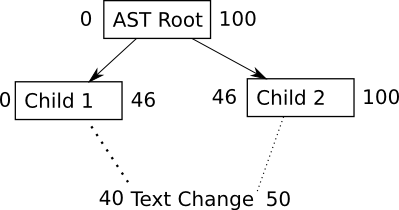
\includegraphics[scale=1]{DrilldownEx}
 \end{center}
 \caption{An AST showing an partial overlap between child 2 and a text change and child 3 and a text change}
 \label{fig:troubleASTNode}
\end{figure}

In the situation where only part of and AST Node contains the text change the children of that AST Node are examined to see if they are fully within the text change.  If not it keeps recursively checking until either a child falls completely outside the change or is completely in the change.  In the case where a text change is not represented by an AST node then the portion that is not covered by an AST change is deemed to be solely a text based changed.  Items that could be a text based change are comments and white space items.

In some instances items within the text change will not have a corresponding AST node.  These are of interest to us because these are instances where the text may have been changed but it has no impact on the behaviour of the program.  The most likely instances of this is when a comment has changed or if white space has been introduced in the middle of source code. Once the AST node for both revisions has been matched with the text change we can compare the AST nodes and their children to discover if they would behave in the same fashion. If they do behave in the same fashion it could indicate that the change is an ascetic one.

Another change we are interested in is if items have been moved.  We would notice this if there is a both insert and a delete for similar AST node types within the same scope.  If a method has been shifted within a class we would notice similar AST nodes, one being deleted at one location, the other being inserted at a different location.  This is another example of a text based change that does not change the behaviour of the program.

%If we can keep track of renaming

If we find examples of text based changes that do not change the programs' behaviour we have an indication that we can reduce the amount of changes necessary to update another view. This in turn could indicate that we would have less merge conflicts by reducing the overall number of changes.

% In order to do this the source code needs to be divided into understandable 
% sections. When each of these sections for each revising are compared it is 
% possible to determine if a section has been moved.  This enhances what can 
% be detected when examining the differences between two files.
% 

\section{What the tool does}
% answer what it does and how

By checking to see if an insert at one point matches a delete at another point it is possible to detect to see if the code block has moved. In order to determine if the move is one that has no impact the matches are only counted if a match can be found within the same container.  Here, a container is an enclosing scope within the source code, such as a class. For example if a method has been shifted within the same class the program will still act the same.  If a method is moved from one class into an inner class there is no guarantee that they will be evaluated to determine if there is a suitable match.  If a method is shifted from one class to an inner class however the programs' behaviour could have changed.

It is possible that an item has moved and has also been modified.  When this happens we are not able to directly compare items to see if they are equal.  Instead we have to match the items that are the most alike.   
To do this each possible match is given a score which indicates how much they differ from each other.  The score is calculated differently for text based comparisons and AST node comparisions.  

For ast node comparisons we recursively examine the differences beween the child nodes of the items we are comparing.  If an extra child AST node has been inserted or a child AST node is deleted then the default amount is added to the score for the match we are evaluating. If a child AST node has been modified it is the equivalent of both a child AST node being inserted and one being deleted. For this reason the default amount is added to score for the match once for the insertion and once for the removal of the a child AST node.In the example in Figure ~\ref{fig:matchComp} two AST node are being compared with each other. Both the red AST node and the yellow AST node have been removed and a green and an orange node have been inserted.  There has been a total of 4 changes to this level of the AST. 

% need more here

\begin{figure}[!t]
 \begin{center}
 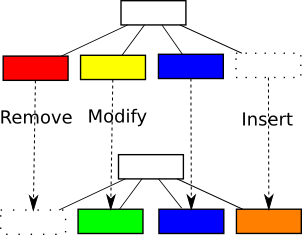
\includegraphics[scale=1]{matchComp}
 \end{center}
 \caption{Two AST nodes being compared to each other by comparing the differences in their child nodes.}
 \label{fig:matchComp}
\end{figure}


Once the various matches have been tested we use a greedy algorithm to select the lowest score for each item.  Once two items are matched with each other both of them can no longer be matched with anything else. The matched items are removed and the next lowest score for a match is evaluated.  To ensure that anything cannot be matched with anything once all good matches are eliminated once the lowest score remaining is greater than the default score of 1000 then any further matches are ignored.  The two items that could have otherwise been matched will remain a solitary insert and a delete.

To a limited extent the Refactor Categories Tool can also deal with renaming. It does this by examing the node and seeing if its children have remained the same and its type remain the same but its name has changed. It can not analyse nodes where the name has not changed as these are not picked up by the initial text comparison.

The Refactor Categories Tool first does a cursory examination of the text differences between two files. It then examines both the differences in executable Java code and the differences between comments and white-space. 



\section{Performance}
As we are testing the complete revision history for several projects there is a high number of changes.  This means that performance is an issue especially for large software projects that have many changes. This means we have not only had to look at using more memory for the Refactor Categories Tool but also had to make some changes to the code to free up more memory where required.

\begin{description}
 \item [By setting object references back to null when they are no longer used.]
  Once a difference has been detected we attempt to remove any of the information we are not going to use in the future.  This should help the garbage collector free up memory. We do this by setting the AST nodes recorded against a difference to null once the difference has been discovered. 
\item [By not analyzing AST node that did not have a text based change.] 
  By ignoring AST nodes and any of their child nodes that do not have a text based change comparing all the AST nodes can be avoided.  This will also help to speed up analysis as these nodes do not need to be analyzed to see if they match.
\item [By comparing only successive changes.] 
  There are a greater amounts of changes if we compare the head against a very old revision. By checking against successive we reduce the number of changes. This also could mean that we need to parse fewer files.
\item [matching within only the required scope.]
  If we were not testing for moves in the same scope we would need to test every deleted AST node against every inserted AST node for the entire file. By stipulating that we can only be sure if it is a legal move if it is in the same scope we not only eliminate a lot of relocations of source code that are illegal but also reduce the number of items that need to be compared. In addition to this the AST node along with its type are recorded in a hash map.  This ensures that only AST nodes that are a similar type are compared against each other.
\end{description}

% future work: by keeping track of equivalencies there is no need to retest
% using the AST

\section{Design decisions}
Java was chosen as both the language to write the tool in and to be the language that the tool would recognise.  This was done as it was a language we understood and to make use of JDime if it was going to be part of the tool.  We wanted to use git due to its distributed nature.  The reasons for choosing a distributed version control system was that we wanted each private view being able to function on its own as a fully fledged project without being dependant on a server.  As we were already using Java rather than using the main Git distribution which is written in C we needed to use JGit instead.    

It turned out we were not able to use JDime because of the issues discussed earlier. Instead we used JastAddJ the same java implementation that JDime uses so that we could implement some of the differences we required including being comment aware and only examining each of the copies of source code.

There are a number of design differences between JDime and the Refactor Categories Tool.  Instead of doing a text comparison first and only proceeding to analyze the program using an AST if there are conflicts the categorization tool examines all files that have a difference in them.  Although this takes longer and is more memory intensive there are some advantages to this. The main advantage is related to the concept of keeping branches as consistent as possible whenever there is a change. An example of this advantage is if a merge was done using an ordinary text comparison and there is a non functional change to only one revision. Examples of a non functional change could include reordering methods or inserting a comment.  As the changes were only done to one of the revisions there is no conflict and JDime only does a text based merge.  During this text based merge, in addition to any of the changes to functionality that we want, we get the non functional changes that change the source code without changing the programs' behaviour. By examining all changes irrespective of if the text has conflicts means that the Refactor Categories Tool can determine if it is a change that would not affect the behaviour of a program.

As there is a cost overhead with testing all the changes rather than just the conflicting ones the categorization tool needs to be efficient in how it tests changes.  Assuming that changes occur in select areas within the file there are portions of the file that have not been changed.  We have developed a method that spends a smaller amount time in  within the portions that have already been identified as not containing changes.  Like JDime we initially do a text based merge.  The text based merge we use however uses the histogram merge in JGit.  This allows us to use information from the text based merge when we analyze the AST tree.  The information used is the ranges of line numbers and operations identified by the histogram merge. The change set has been taken from the original JGit based diff contains the start and end of the change in both files and what type of change it is (insert delete or modify).  By reusing these ranges of line numbers it is possible to figure out which AST items these changes affect. This is done by loading the file into the JastAddJ parser to get an AST tree. Line numbers for each item in the tree are then compared to line numbers from the change set. The line numbers are matched to the position information stored in each AST node using the following method.

The root of the AST is identified as the AST node we need to start at. 
We only begin any analysis, if the AST node resides completely within a block of text changes.
If there are any separate blocks of changes that occur between the start position of the AST node and the end position of the AST node then we recursively examine the AST nodes children.

% The Refactor Categories Tool first works out which text has changed using 
% the same method as JGit.
% This initial examination returns the differences based on a line by line 
% basis rather than using a smaller granularity.
% This means that the set of changes found could still contain code that is 
% comparatively the same.
% The set of changes found in using the JGit histogram comparison are then 
% evaluated.
% The reason for this is that some items of text could be in a differing order 
% but still be a valid Java program
% 
% 
% In order to resolve some limitations with JDime and the text only merge in 
% GIT information about which line numbers are retained after the first text 
% merge.  In JDime these are ignored and the AST is relied upon to hold all 
% the information.


% after finished drill down we have a record of the same changes as JGit
% except now we also have the ASTs

In some instances there is no position information stored in the JastAddJ AST nodes.  This could be because they are generated by the parser to reflect parts of the Java language that are inferred rather than directly mentioned in the code.  An example of this would be the use of super in the constructor.  Even if it is not written in the code for every constructor has a super. Likewise all methods mentioned in an interface have a public type even if is not in the code.

To get around this problem we have needed to discover the end position of the previous AST Node to determine the position the inferred AST node should occupy.  This means that the inferred AST node is in the right position but is not represented by a block of text in the source code. 

Comment and white-space are also examined separately as they also could give some indication of where code has been moved from or to.
Before being checked to find matches unnecessary white-space is identified and recorded.
Any text that remains is examined to determine if its is a comment. 

Because of the way we are using the position in the code to identify AST nodes there are circumstances when parts of the Java programming language are identified as being surplus text. These have already been identified and represented as an AST Node. By identifying comments we can eliminate any of the items falsely recorded as comments.

% Comments and white-space cannot be shown in the AST tree so they need to be
% dealt with separately

% comparing AST nodes
% the matcher and how using a score works
% finding the best match
% 
% 
% explain how we limit matching just to the parent of the thing being matched

Rather than comparing everything with each other to determine matches it is more efficient to match just the items that are under the same AST structure.  This means that it is more likely that we get a match that is going to be relevant and valid.  An example of this is matching methods. If the methods are under the same container (a class) they may be legally swapped without causing issues.  If the method has been moved to an inner class from an outer one however it becomes more complicated and we cannot guarantee that the code is equivalent.  


\section{Limitations of the tool}
The Refactor Categories Tool focuses only on areas where there has been a text change in the source code. 
It is harder to investigate any change that has causes side effects in unchanged code.  Fortunately it is not often that this type of side effect will be purposely placed in the code as it reflects bad design decisions.  This may however be an issue with bugs, which are unintentionally occur in the code.  
This also means that the Refactor Categories Tool will not be able to tell when some code has been copied but the original remains unchanged. Instead it will assume that it is a completely new insertion of code.

If a change of a variable name is noticed the program still retains the same behaviour if the rename operation has worked on all instances where the old name was previously used.  As we do not examine parts of the code that have not experienced a text based change we cannot guarantee that a rename operation is a valid one. We have an indication that it might be if the code still compiles without error. If a variable name is changed to that of an already existing variable however the behavior of the program could change. This is known as a \emph{semantic conflict}.  This issue already exists in a text based merge and Fan \cite{Fan2012}, Shao \cite{Shao2009} and others address this issue. 


\chapter{Experimental Results}

\section{Purpose}
The purpose of this experiment is to measure how many insertions, deletion and modifications are performed on the Java AST verses comments across a range of realistic benchmarks. Similarly, how many insert and delete pairs can be classified as moves. 

% establish if there are superficial changes in currently working projects.  
% By superficial we mean that the change does not add much of value apart from 
% personal taste or formatting.  In some cases changes to the order of methods 
% within a class does change the behaviour of a program, this is an example of 
% a superficial change.  It is harder to determine if comments are superficial 
% because certain comments could be important to others and others irrelevant. 
% We will attempt to establish if there are any patterns in comments to 
% determine if they are superficial or not.  Determining if there are 
% superficial change may indicate that there is a separation between personal 
% preferences that would be best contained in a private view and items that 
% need to be shared for collaboration.

\section{Methodology}
We will now outline the experimental methodology. Our goal is make it possible for someone to reproduce our experiment.

The experiment was run on a Lenovo laptop with 3.5GB Ram and 113.2 GB disk space assigned to the 64 bit Ubuntu 13.10 (Saucy Salamander) operating system. The tests were written in Java and run within the Eclipse IDE



 
 
 \begin{table}[H]
    \small{
    \begin{tabular}{l|lllll}
    Benchmark        & Description   & Commits  & LOC   \\ \hline
    Jasm             &  \begin{minipage}[t]{0.5\textwidth}
Java bytecode assembler written for use with the Whiley programming language.

github.com/Whiley/Jasm 
\end{minipage}        & 74      & 29139 \\
    Jpp              & \begin{minipage}[t]{0.5\textwidth}
    Pre-processor for Java based on Bash shell script.
    
github.com/maandree/jpp
\end{minipage}        & 40      & 254   \\
    AST Java         & \begin{minipage}[t]{0.5\textwidth}
    Small parser written to transform Java into an AST.
    
github.com/klangner/ast-java 
\end{minipage}       & 24      & 10174 \\
\begin{minipage}[t]{0.15\textwidth}Java Object Diff\end{minipage} & \begin{minipage}[t]{0.5\textwidth}
Allows two Java objects to be compared at runtime.
     
github.com/SQiShER/java-object-diff 
\end{minipage}        & 291     & 10023 \\
    DiffJ            & \begin{minipage}[t]{0.5\textwidth}
    Diff tool which in addition to ignoring white space ignores changes of ordering in package names for a Java file.
    
github.com/jpace/diffj
\end{minipage}        & 490     & 13712 \\
    IRE              & \begin{minipage}[t]{0.5\textwidth}
    Java library for regular expression matching.
    
github.com/jkff/ire  
\end{minipage}       & 41      & 2714  \\
    Syntax           & \begin{minipage}[t]{0.5\textwidth}
    Compiler compiler used for teaching. 
    
github.com/jaimegarza/syntax 
\end{minipage}        & 89      & 9376  \\

    Auto Refactor           & \begin{minipage}[t]{0.5\textwidth}
    Eclipse plug-in that automatically refactors code 
    
github.com/JnRouvignac/AutoRefactor 
\end{minipage}        & 212      & 13400  \\
    \end{tabular}
    }
\end{table}
 
% 
% The Refactor Categories Tool analyses all the historical changes ever made 
% on a software project by extracting successive revisions from a Git 
% repository using JGit.  Once we have two revisions we need to compare them.  
% To do this we compare each of the Java files in both revisions one by one. 
% We only test the Java file if it has been modified or renamed.  If the file 
% been inserted or deleted we ignore it because there is no way to make a 
% comparison. Once we have established that Java files exist, both in the 
% original and the updated copy, we use the text diff in JGit to compare them. 
% As outlined in section \ref{matchingTextWithAST} we figure out which AST 
% nodes the text changes contain.
% The Refactor Categories Tool splits up the identified blocks of source code 
% into several AST nodes and identifies anything between AST Nodes as being 
% text. @c
This text is further evaluated to determine if it is a change to comments or a change to white space. 
An example of this is if the text comparison detects a single change that inserts two new methods and a comment.  
The Refactor Categories Tool will recognise this as three distinct changes. 
This means that it is possible for the Refactor Categories Tool to notice more changes than a text based comparison. 

We had some garbage collection memory issues with some benchmarks that we were testing. 
To resolve these issues the Refactor Categories Tool was run individually once for each benchmark to further ensure that there were no memory leaks between runs.
We also increased the memory by changing the parameters for the run configuration.  The following parameters were added to the run configuration for the test.

\begin{verbatim}
-Xms512M 
-Xmx4096M
\end{verbatim}



% There are a number of comparison operations that the refactor categories 
% tool investigates
% 
% \begin{description}
% 
%   \item [Delete]
%   <<del>>
%   \item [Insert]
%   <<ins>>
% 
%   \item [Modify]
%   <<mod>>
%   \item [Move]
%   <<mov>>
%   \item [Rename]
%   <<ren>>
%   \item [Equivalent]
%   <<eqv>>
% \end{description}
%  @c
% renames are determined as being something where although the AST label has 
% changed the type of the AST node remains the same and its contents have not 
% been changed in any way.



\section{Results}
\subsection{Overview}
After running the Refactor Categories tool over our benchmark suite we obtained the results shown in Table \ref{tab:results}



\begin{table}[t!]
    \small
    \begin{tabular}{l|llllll|l|lll}
    Benchmark        & \multicolumn{6}{|c|}{Java}           & WS & \multicolumn{3}{|c}{Comments} \\ \cline{2-7} \cline{9-11}
    ~                & Ins  & Del  & Mod  & Mov & Ren & Eqv & ~          & Ins      & Del & Mod  \\ \hline
    Jasm             & 264  & 76   & 385  & 7   & 0   & 0   & 26         & 7        & 6   & 95   \\
    Jpp              & 43   & 9    & 50   & 0   & 0   & 0   & 6          & 1        & 2   & 11   \\
    AST Java         & 87   & 28   & 72   & 1   & 0   & 11  & 5          & 2        & 0   & 22   \\
    \begin{minipage}[t]{0.15\textwidth}Java Object Diff\end{minipage} & 2645 & 1961 & 8862 & 5   & 9   & 183 & 277        & 14       & 39  & 1438 \\
    DiffJ            & 3106 & 3164 & 5192 & 58  & 82  & 18  & 276        & 36       & 39  & 291  \\
    IRE              & 263  & 213  & 640  & 1   & 2   & 30  & 49         & 10       & 3   & 79   \\
    Syntax           & 1142 & 544  & 2216 & 6   & 7   & 12  & 204        & 14       & 81  & 451  \\
    Auto refactor    & 1702 & 1621 & 2809 & 7   & 16  & 25  & 295        & 30       & 16  & 568  \\
    \end{tabular}
    \caption{Results over our benchmark suite showing the number of inserts (INS), deletes (DEL), modifications (MOD), moves (MOV), renames (REN) and equivalences (EQV) for Java AST, comments and white-space (WS) changes}
    \label{tab:results}
\end{table}

The number of text changes that were recognised during text comparison for each benchmark are shown in Table \ref{tab:textcomp}. Note that the values in this table are lower as the Refactor Categories tool detects multiple changes which a text based comparison aggregates.  

\begin{table}[H]
    \centering
    \begin{tabular}{l|lll}
    Benchmark        & \multicolumn{3}{|c}{Text Diff} \\ \hline
    ~                & Ins            & Del & Mod  \\ \hline
    Jasm             & 91             & 44  & 337  \\
    Jpp              & 23             & 3   & 41   \\
    AST Java         & 44             & 15  & 85   \\
    Java Object Diff & 1186           & 837 & 8219 \\
    DiffJ            & 746            & 991 & 3544 \\
    IRE              & 112            & 49  & 465  \\
    Syntax           & 691            & 214 & 1863 \\
    Auto Refactor    & 639            & 309 & 1621 \\
    \end{tabular}
    \caption{The result of doing an ordinary text comparison showing the number of inserts (INS), deletes (DEL) and modifications (MOD)}
    \label{tab:textcomp}
\end{table}



\subsection{Discussion}
Figure \ref{fig:textDifference} show the average for all the benchmarks of the types of operations found during an ordinary text comparison.  
The most common merge operation is when items have been modified.  
This occured on average  almost 73 percent of the time.

\begin{figure}[!t]
 \begin{center}
 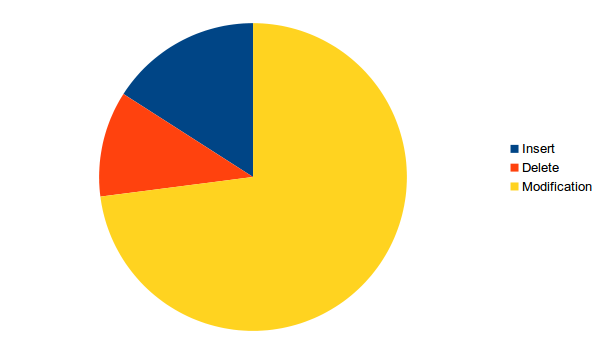
\includegraphics[scale=.8]{TextDifference}
 \end{center}
 \caption{Type of operations for an ordinary text comparision on average for all the benchmarks}
 \label{fig:textDifference}
\end{figure}

When we examine the Java AST differences for the same benchmark however the number of modifications reduces and the number of insertions and deletes increase.
This is shown in Figure \ref{fig:javaDifference}.
The reason for this is because an change done to block of text recorded in the \lstinline{EditList} object is made up of a number of smaller changes.  
If the block of text is a delete all the smaller changes are also delete.  
The same is true for inserts, all the smaller changes will also be inserts.
With a modified block of text modifications however the smaller changes could be inserts, deletes or modifications.
What this means is that some of the changes that an ordinary text diff recognises as modifications could actully made up of individual inserts and deletes. 

\begin{figure}[!t]
 \begin{center}
 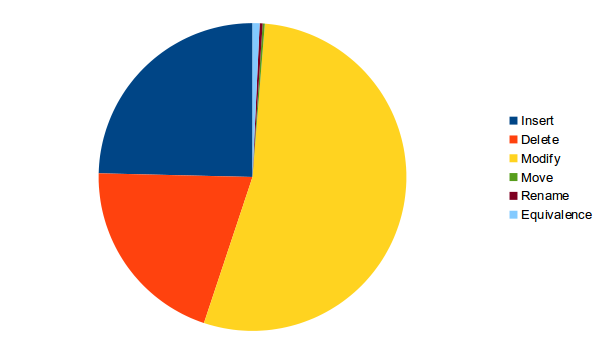
\includegraphics[scale=.8]{JavaDiff}
 \end{center}
 \caption{Type of operations for an ordinary text comparision on average for all the benchmarks}
 \label{fig:javaDifference}
\end{figure}

Most of the changes where still identified as modifications rather than moves, renames or changes to comments. 
There are enough of the changes to comments and moves of the code however to warrent further investigation.

% resons why these benchmarks where used
% 
% 

% There were a number of benchmarks we would have liked to have used but due 
% to memory constraints we had to omit these from the benchmark suite.
% 
% 
% 
%  \begin{table}[H]
%     \small{
%     \begin{tabular}{l|lllll}
%     Benchmark        & Description   & Commits  & LOC   \\ \hline
%     Antlr4             &  \begin{minipage}[t]{0.5\textwidth}
%     A parser generator used to create programming grammers.
% 
% github.com/antlr/antlr4
% \end{minipage}        & 2867      & 40373 \\
% 
%     Clojure             & \begin{minipage}[t]{0.5\textwidth}
%     A programming language that targets the JVM
% github.com/clojure/clojure
% \end{minipage}        & 2602      & 37512   \\
%     gitblit         & \begin{minipage}[t]{0.5\textwidth}
%      Java implementation of Git.
% github.com/gitblit/gitblit
% \end{minipage}       & 2334       & 72188 \\
%     Jacoco            & \begin{minipage}[t]{0.5\textwidth}
%     Library used to determine code coverage.
% github.com/jacoco/jacoco
% \end{minipage}        & 1184     & 25357 \\
%     JGit             & \begin{minipage}[t]{0.5\textwidth}
%     Java implementation of Git developed by the Eclipse Foundation.
% eclipse.org/jgit
% \end{minipage}       & 3285      & 137993  \\
%     Lombok           & \begin{minipage}[t]{0.5\textwidth}
%     A library that used annotaions to extend Java.
% github.com/rzwitserloot/lombok
% \end{minipage}        & 1624      & 39154  \\
%     Revori           & \begin{minipage}[t]{0.5\textwidth}
%     A revision based DBMS.
% github.com/ReadyTalk/revori
% \end{minipage}        & 349      & 18931  \\
%     \end{tabular}
%     }
% \end{table}
% 

% 
% 
% Memory issues
% baselines we could not compare
% the graeter the amount of revisons the more chance that there was a memeory 
% error
% 
% 
% Moves
% Renames
% comment deletion /inserts and modifications
%   the largest change

There were some interesting results for JDiff

% The data sets following are complete git repositories which have been 
% examined to discover the proportion of changes to behaviour compared to 
% ascetic changes that do not affect the behaviour of the program.
% 
% 
% in table ~\ref{tab:DataSets}
% 
% \begin{table}
%   \caption{Complete git repositories that are tested}
%   \label{tab:DataSets}
%   \begin{center}
%     \begin{tabular}{|c|c|c|}
%        Jasm & this a a Java bytecode assembler
%        written for use with the Whiley programming language. & 
% https://github.com/Whiley/Jasm\\
%       foo & bar \\
%     \end{tabular}
%   \end{center}
% \end{table}
% 

% 
% 
% 
% There are a number of Java categories that the Refactor Categories Tool will 
% recognise.  Apart from the traditional insert, delete and modify it will 
% also recognise if an AST Node has been renamed but the content and type of 
% the node remains the same.  It will recognise valid moves within a scope. It 
% will also recognise when the text based merge got it wrong by claiming that 
% the code was not functionally equivalent when in fact it was.
% 
% Apart from this it will also differentiate between Java code and comments.  
% It can tell if comments have been inserted, modified, moved or deleted.  It 
% will also pick up any changes to that white-space that have not already been 
% figured out by the text based comparison.
 
% Comments
%     Insert
%     Delete
%     Modify
%     Move
% White space
%    Modify
% 
% Java
%  Insert
%  Delete
%  Modify
%  Move
%  Rename


% need the results in here
% 
% 
% what this means
% modifications to comments
% 
% modification to comments could be surplus to need
% 
% 
% Examine certain events
% 
% in this case the comment is removed but as the comment is associated with a 
% functional change the comment also needs to change in both versions



\chapter{Future Work}

Performance of Refactor Categories Tool could be further enhanced by only parsing nodes that are part of the change set or are ancestors of this.  This however would require major changes to the parser or rewriting it. It would save memory in addition to speeding up the parsing of Java code into AST nodes.



% 
% comments need to be able to be associated to blocks of code so that it is 
% possible tyo tell if removing or addin a comment should be reflected in 
% other views when there is a source code change
% 
% removing AST nodes once they have been used
% 
% future work: by keeping track of equivalencies there is no need to retest 
% using the AST
% 
% To reuse the refactor categories tool or something similar to create 
% seperate views as envisaged
% 
% 








\chapter{Conclusions and future work}\label{C:con}

In this thesis we presented the concept of maintaining private views in Java.
A private view presented here is an environment that allows a developer to import changes they want while avoiding hidden unwanted changes. 
This concept would also allow programmers to implement lightweight refactoring to their tastes, while minimising the impact on others.  
In evaluating what these private view will look like we used version control systems as a starting point.
There are some features of version control systems that already temporarily limit unwanted changes (e.g. branches).
However, during a merge any unwanted refactoring is imported. 
To this end we created the Refactor Categories Tool as a precursor to creating private views. 
This tool analyses the difference between two revisions such as encountered during a commit and identifies some examples of lightweight refactoring.
The way that the Refactor Categories Tool analyses these differences is by first parsing the source for both commits into a Java Abstract Syntax Tree (AST).
Once the AST is populated we then identify which parts of the AST match the differences we want to examine.
We then use the AST to identify additional features that have been changed. 
The features we have focused on are ones that do not change any functionality such as methods being moved or comments being changed. 
The results show that some of these lightweight refactorings are encountered in practice.
As the Refactor Categories Tool is a prototype it did not, unfortunately, select as many as we hoped.
We believe that it is possible to detect many more non-functional changes using more advanced identification algorithms.

\section{Future work}

In order to further the research into private views it would be useful to evaluate how the Refactor Categories Tool could be enhanced to detect more non functional changes. 
In addition to this some other tools could be adapted to create and evaluate the usefulness of private views.  
\subsection{Changes to the Refactor Categories Tool}

There are a number of ways that the Refactor Categories Tool could be changed to discover more moves, and renames:

\begin{itemize}

  \item At the moment the Refactor Categories Tool only examines moves that occur within a class, however, there could be non-functional changes that occur inside a method. 
An example would be if a local variable declaration was moved.
Sometimes this move would have no effect on the code and others it could cause the code to no longer compile.
  
  \item At the moment the refactor categories tool only compares matches within a limited scope (i.e. a class).  
  By allowing the Refactor Categories Tool to check other parts of the code, such as inner classes or even other files may also produce some interesting results.
Although we cannot guarantee that the moves discovered are valid ones this could give us more information about the source code we are examining.

  \item At the moment the Refactor Categories Tool only examines files that have been identified by JGit as being modified or renamed.
In some instances JGit could have incorrectly determined that a file as been deleted and reinserted rather than being renamed or moved.
This could happen easily since during a move or rename the a Java file changes the package reference and class name within a file.
This is especially true if the class has both been renamed and modified.

  \item Revising the scoring system for matching up inserts and deletes may produce some better results.
At the moment modifications are counted as two changes using the scoring system to match inserts and deletes.
Experimenting by reducing this value could improve the number of matches.

\end{itemize}




   

In addition to moves and renames, other lightweight refactoring may be of interest.
One of these are changes to access modifiers.
An example would be if a methods access changes from being private to being public.
Each of the method calls would then need to be rechecked to ensure that the change does not affect functionality.
Due to the possibilities of overloaded methods in Java this would be complicated.

An additional lightweight refactoring that could be considered is code that has been duplicated.
This could be done in a similar manner as how the Refactor Categories Tool check for code that has moved.
If we also check for code that has been modified slightly we may be able to determine that a copy and paste has been used to generate new code.
However, at the moment the Refactor Categories Tool only considers code that has been changed.
If we want to analyse where code has been copied we would need to check the entire source for copies as opposed to just the items that have changed.

Comments could be associated with the AST Node they relate to.  
With this change would be possible to tell if changing a comment should be reflected in other views when there is a source code change. 
This change is difficult as it is hard to tell which block of code the comment refers to.  
One way this could be done would be to associate single-line comments at the end of the line with the AST Node that appears directly before them and other comments with the AST node that appears directly after them.  
This however is only a rough approximation so it may be helpful to also be able to specify exceptions to these rules by using annotations that tie the comment to a block of code. Annotations could also be used to specify how important the comment is.
If the comment is marked as unimportant it would indicate that it still should not be considered a change even if it differs between revisions.

The Refactor Categories Tool could be re-purposed to allow it to be used as a merge tool rather than a comparison tool that we are currently using it for.  
This would bring us a step closer to being able to realise the vision of having better separated private views.  

Performance of Refactor Categories Tool could be further enhanced by only parsing nodes that contain the text change.
This however would require major changes to the parser or rewriting it. There would also be the complexity of figuring out how to only partially parse a source code.
The benefits of rewriting the parser would save memory in addition to speeding up the parsing of Java code into AST nodes.


\subsection{Other lines of enquiry}

There are other tools that could be modified to determine when a refactoring has taken place.

JDime has already been investigates as part of this thesis.
Although JDime cannot recognise changes to comments or white-space it could be re-purposed.
If it could be converted into a comparison tool rather than a merge tool then code that has been refactored differently could be compared without the result being normalised.

According to Pace \cite{Pace} \emph{DiffJ} is able to find the functional differences between two revisions of Java source code.
When computing the difference DiffJ ignores a range of lightweight refactorings such as moved methods, moved imports and the code being reformatted. 
As it ignores comments and white-space however, it will not be able to determine if there have been comment based changes that may be important. 



% 
% future work: by keeping track of equivalences there is no need to retest 
% using the AST
% 


%%%%%%%%%%%%%%%%%%%%%%%%%%%%%%%%%%%%%%%%%%%%%%%%%%%%%%%

% and of course book style knows about backmatter
% \backmatter caused problems with appendices :-(
% and of course report style doesn't
%%%%%%%%%%%%%%%%%%%%%%%%%%%%%%%%%%%%%%%%%%%%%%%%%%%%%%%


%\bibliographystyle{ieeetr}
\bibliographystyle{acm}
\bibliography{Thesis}


\end{document}
